\documentclass[1p]{elsarticle_modified}
%\bibliographystyle{elsarticle-num}

%\usepackage[colorlinks]{hyperref}
%\usepackage{abbrmath_seonhwa} %\Abb, \Ascr, \Acal ,\Abf, \Afrak
\usepackage{amsfonts}
\usepackage{amssymb}
\usepackage{amsmath}
\usepackage{amsthm}
\usepackage{scalefnt}
\usepackage{amsbsy}
\usepackage{kotex}
\usepackage{caption}
\usepackage{subfig}
\usepackage{color}
\usepackage{graphicx}
\usepackage{xcolor} %% white, black, red, green, blue, cyan, magenta, yellow
\usepackage{float}
\usepackage{setspace}
\usepackage{hyperref}

\usepackage{tikz}
\usetikzlibrary{arrows}

\usepackage{multirow}
\usepackage{array} % fixed length table
\usepackage{hhline}

%%%%%%%%%%%%%%%%%%%%%
\makeatletter
\renewcommand*\env@matrix[1][\arraystretch]{%
	\edef\arraystretch{#1}%
	\hskip -\arraycolsep
	\let\@ifnextchar\new@ifnextchar
	\array{*\c@MaxMatrixCols c}}
\makeatother %https://tex.stackexchange.com/questions/14071/how-can-i-increase-the-line-spacing-in-a-matrix
%%%%%%%%%%%%%%%

\usepackage[normalem]{ulem}

\newcommand{\msout}[1]{\ifmmode\text{\sout{\ensuremath{#1}}}\else\sout{#1}\fi}
%SOURCE: \msout is \stkout macro in https://tex.stackexchange.com/questions/20609/strikeout-in-math-mode

\newcommand{\cancel}[1]{
	\ifmmode
	{\color{red}\msout{#1}}
	\else
	{\color{red}\sout{#1}}
	\fi
}

\newcommand{\add}[1]{
	{\color{blue}\uwave{#1}}
}

\newcommand{\replace}[2]{
	\ifmmode
	{\color{red}\msout{#1}}{\color{blue}\uwave{#2}}
	\else
	{\color{red}\sout{#1}}{\color{blue}\uwave{#2}}
	\fi
}

\newcommand{\Sol}{\mathcal{S}} %segment
\newcommand{\D}{D} %diagram
\newcommand{\A}{\mathcal{A}} %arc


%%%%%%%%%%%%%%%%%%%%%%%%%%%%%5 test

\def\sl{\operatorname{\textup{SL}}(2,\Cbb)}
\def\psl{\operatorname{\textup{PSL}}(2,\Cbb)}
\def\quan{\mkern 1mu \triangleright \mkern 1mu}

\theoremstyle{definition}
\newtheorem{thm}{Theorem}[section]
\newtheorem{prop}[thm]{Proposition}
\newtheorem{lem}[thm]{Lemma}
\newtheorem{ques}[thm]{Question}
\newtheorem{cor}[thm]{Corollary}
\newtheorem{defn}[thm]{Definition}
\newtheorem{exam}[thm]{Example}
\newtheorem{rmk}[thm]{Remark}
\newtheorem{alg}[thm]{Algorithm}

\newcommand{\I}{\sqrt{-1}}
\begin{document}

%\begin{frontmatter}
%
%\title{Boundary parabolic representations of knots up to 8 crossings}
%
%%% Group authors per affiliation:
%\author{Yunhi Cho} 
%\address{Department of Mathematics, University of Seoul, Seoul, Korea}
%\ead{yhcho@uos.ac.kr}
%
%
%\author{Seonhwa Kim} %\fnref{s_kim}}
%\address{Center for Geometry and Physics, Institute for Basic Science, Pohang, 37673, Korea}
%\ead{ryeona17@ibs.re.kr}
%
%\author{Hyuk Kim}
%\address{Department of Mathematical Sciences, Seoul National University, Seoul 08826, Korea}
%\ead{hyukkim@snu.ac.kr}
%
%\author{Seokbeom Yoon}
%\address{Department of Mathematical Sciences, Seoul National University, Seoul, 08826,  Korea}
%\ead{sbyoon15@snu.ac.kr}
%
%\begin{abstract}
%We find all boundary parabolic representation of knots up to 8 crossings.
%
%\end{abstract}
%\begin{keyword}
%    \MSC[2010] 57M25 
%\end{keyword}
%
%\end{frontmatter}

%\linenumbers
%\tableofcontents
%
\newcommand\colored[1]{\textcolor{white}{\rule[-0.35ex]{0.8em}{1.4ex}}\kern-0.8em\color{red} #1}%
%\newcommand\colored[1]{\textcolor{white}{ #1}\kern-2.17ex	\textcolor{white}{ #1}\kern-1.81ex	\textcolor{white}{ #1}\kern-2.15ex\color{red}#1	}

{\Large $\underline{12a_{0853}~(K12a_{0853})}$}

\setlength{\tabcolsep}{10pt}
\renewcommand{\arraystretch}{1.6}
\vspace{1cm}\begin{tabular}{m{100pt}>{\centering\arraybackslash}m{274pt}}
\multirow{5}{120pt}{
	\centering
	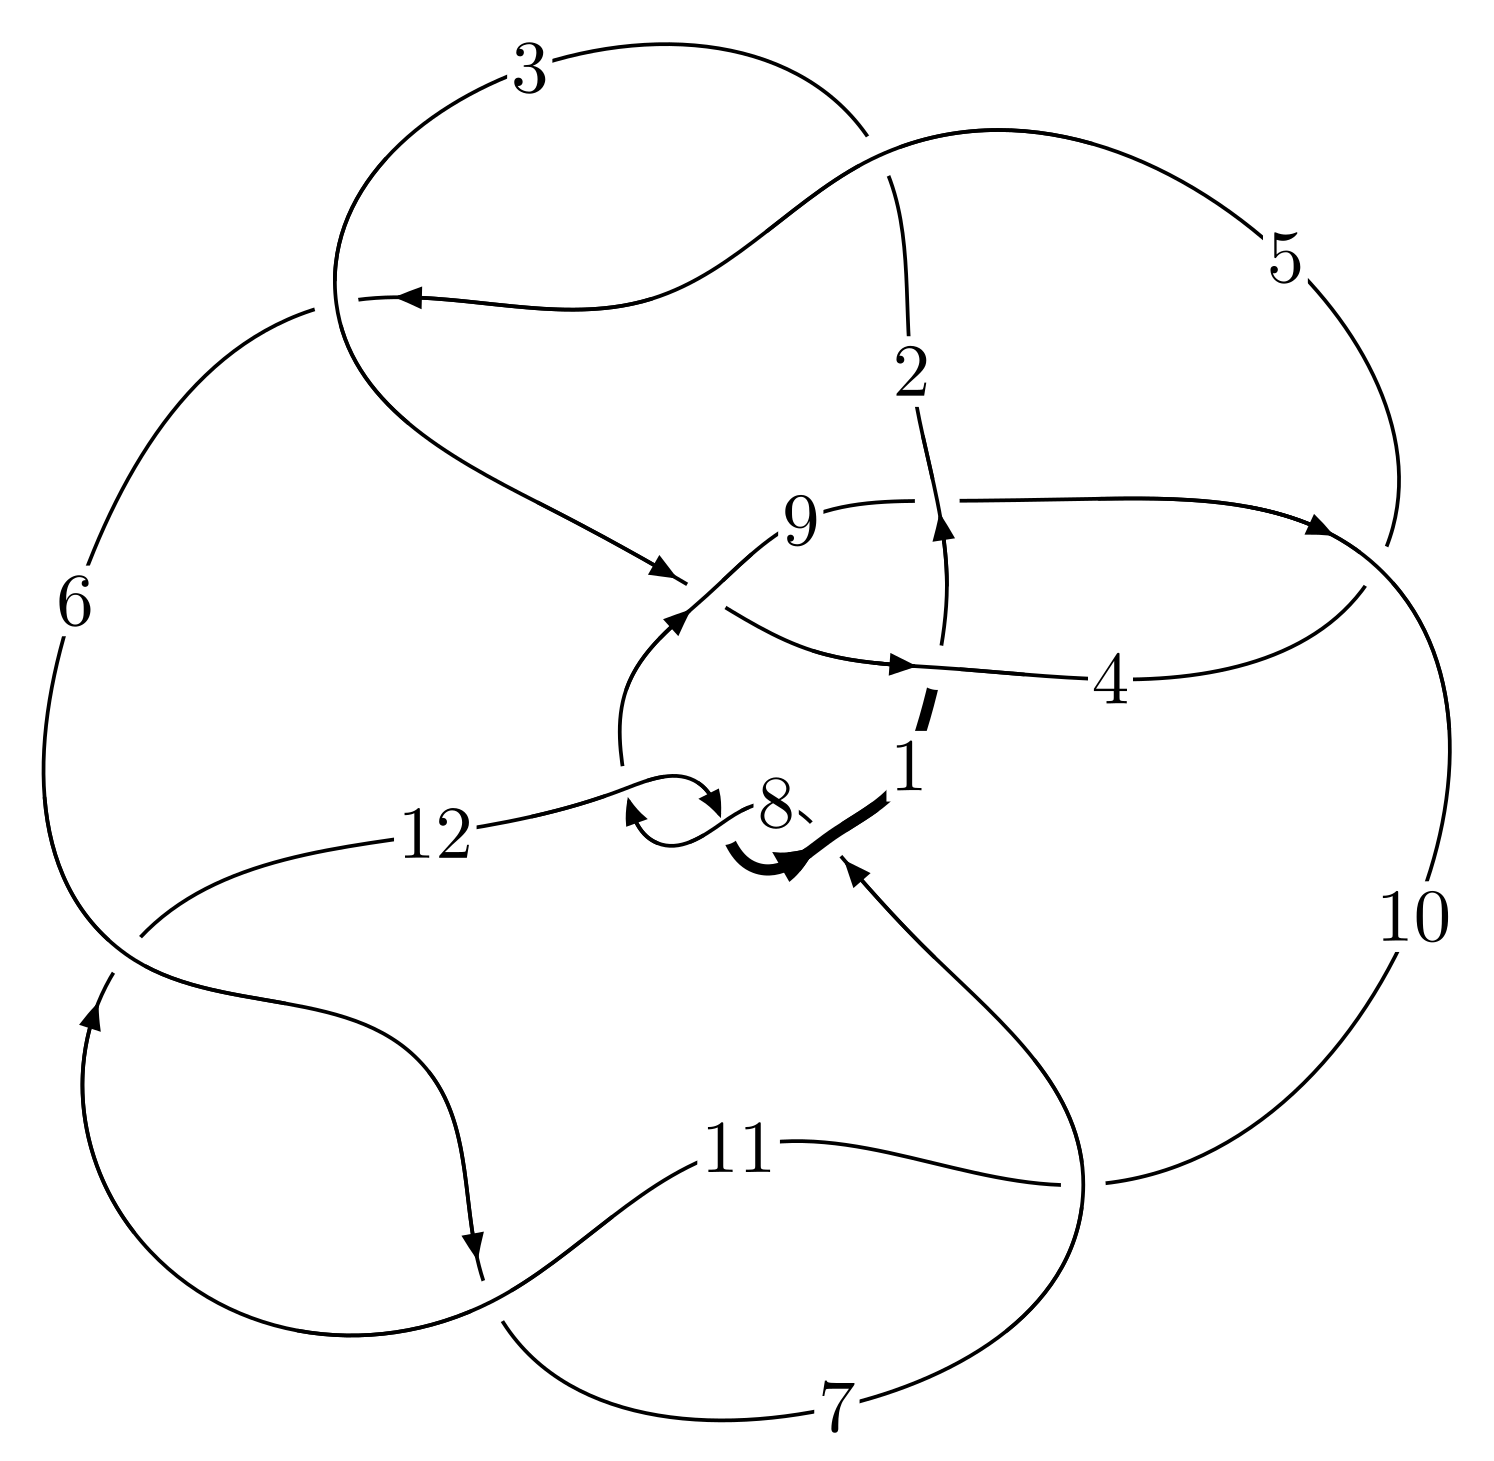
\includegraphics[width=112pt]{../../../GIT/diagram.site/Diagrams/png/1654_12a_0853.png}\\
\ \ \ A knot diagram\footnotemark}&
\allowdisplaybreaks
\textbf{Linearized knot diagam} \\
\cline{2-2}
 &
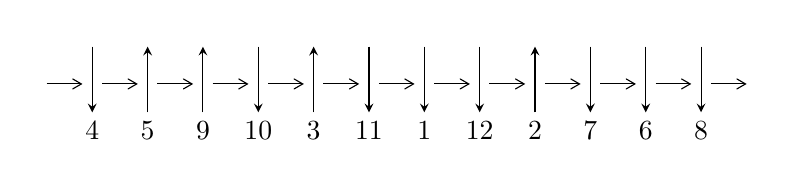
\begin{tikzpicture}[x=20pt, y=17pt]
	% nodes
	\node (C0) at (0, 0) {};
	\node (C1) at (1, 0) {};
	\node (C1U) at (1, +1) {};
	\node (C1D) at (1, -1) {4};

	\node (C2) at (2, 0) {};
	\node (C2U) at (2, +1) {};
	\node (C2D) at (2, -1) {5};

	\node (C3) at (3, 0) {};
	\node (C3U) at (3, +1) {};
	\node (C3D) at (3, -1) {9};

	\node (C4) at (4, 0) {};
	\node (C4U) at (4, +1) {};
	\node (C4D) at (4, -1) {10};

	\node (C5) at (5, 0) {};
	\node (C5U) at (5, +1) {};
	\node (C5D) at (5, -1) {3};

	\node (C6) at (6, 0) {};
	\node (C6U) at (6, +1) {};
	\node (C6D) at (6, -1) {11};

	\node (C7) at (7, 0) {};
	\node (C7U) at (7, +1) {};
	\node (C7D) at (7, -1) {1};

	\node (C8) at (8, 0) {};
	\node (C8U) at (8, +1) {};
	\node (C8D) at (8, -1) {12};

	\node (C9) at (9, 0) {};
	\node (C9U) at (9, +1) {};
	\node (C9D) at (9, -1) {2};

	\node (C10) at (10, 0) {};
	\node (C10U) at (10, +1) {};
	\node (C10D) at (10, -1) {7};

	\node (C11) at (11, 0) {};
	\node (C11U) at (11, +1) {};
	\node (C11D) at (11, -1) {6};

	\node (C12) at (12, 0) {};
	\node (C12U) at (12, +1) {};
	\node (C12D) at (12, -1) {8};
	\node (C13) at (13, 0) {};

	% arrows
	\draw[->,>={angle 60}]
	(C0) edge (C1) (C1) edge (C2) (C2) edge (C3) (C3) edge (C4) (C4) edge (C5) (C5) edge (C6) (C6) edge (C7) (C7) edge (C8) (C8) edge (C9) (C9) edge (C10) (C10) edge (C11) (C11) edge (C12) (C12) edge (C13) ;	\draw[->,>=stealth]
	(C1U) edge (C1D) (C2D) edge (C2U) (C3D) edge (C3U) (C4U) edge (C4D) (C5D) edge (C5U) (C6U) edge (C6D) (C7U) edge (C7D) (C8U) edge (C8D) (C9D) edge (C9U) (C10U) edge (C10D) (C11U) edge (C11D) (C12U) edge (C12D) ;
	\end{tikzpicture} \\
\hhline{~~} \\& 
\textbf{Solving Sequence} \\ \cline{2-2} 
 &
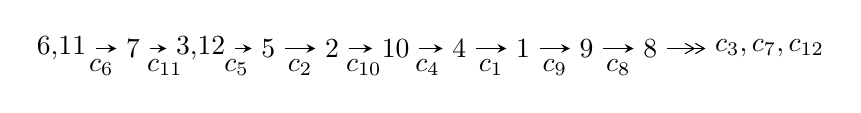
\begin{tikzpicture}[x=23pt, y=7pt]
	% node
	\node (A0) at (-1/8, 0) {6,11};
	\node (A1) at (1, 0) {7};
	\node (A2) at (33/16, 0) {3,12};
	\node (A3) at (25/8, 0) {5};
	\node (A4) at (33/8, 0) {2};
	\node (A5) at (41/8, 0) {10};
	\node (A6) at (49/8, 0) {4};
	\node (A7) at (57/8, 0) {1};
	\node (A8) at (65/8, 0) {9};
	\node (A9) at (73/8, 0) {8};
	\node (C1) at (1/2, -1) {$c_{6}$};
	\node (C2) at (3/2, -1) {$c_{11}$};
	\node (C3) at (21/8, -1) {$c_{5}$};
	\node (C4) at (29/8, -1) {$c_{2}$};
	\node (C5) at (37/8, -1) {$c_{10}$};
	\node (C6) at (45/8, -1) {$c_{4}$};
	\node (C7) at (53/8, -1) {$c_{1}$};
	\node (C8) at (61/8, -1) {$c_{9}$};
	\node (C9) at (69/8, -1) {$c_{8}$};
	\node (A10) at (11, 0) {$c_{3},c_{7},c_{12}$};

	% edge
	\draw[->,>=stealth]	
	(A0) edge (A1) (A1) edge (A2) (A2) edge (A3) (A3) edge (A4) (A4) edge (A5) (A5) edge (A6) (A6) edge (A7) (A7) edge (A8) (A8) edge (A9) ;
	\draw[->>,>={angle 60}]	
	(A9) edge (A10);
\end{tikzpicture} \\ 

\end{tabular} \\

\footnotetext{
The image of knot diagram is generated by the software ``\textbf{Draw programme}" developed by Andrew Bartholomew(\url{http://www.layer8.co.uk/maths/draw/index.htm\#Running-draw}), where we modified some parts for our purpose(\url{https://github.com/CATsTAILs/LinksPainter}).
}\phantom \\ \newline 
\centering \textbf{Ideals for irreducible components\footnotemark of $X_{\text{par}}$} 
 
\begin{align*}
I^u_{1}&=\langle 
1.02805\times10^{16} u^{42}-1.52246\times10^{16} u^{41}+\cdots+1.26321\times10^{17} b-8.98707\times10^{16},\\
\phantom{I^u_{1}}&\phantom{= \langle  }-7.21225\times10^{16} u^{42}+3.40792\times10^{16} u^{41}+\cdots+1.68428\times10^{17} a-9.26394\times10^{16},\;u^{43}- u^{42}+\cdots- u-1\rangle \\
I^u_{2}&=\langle 
2.49774\times10^{62} u^{57}-1.12667\times10^{62} u^{56}+\cdots+3.57909\times10^{63} b-1.55315\times10^{63},\\
\phantom{I^u_{2}}&\phantom{= \langle  }3.07126\times10^{63} u^{57}-3.20268\times10^{64} u^{56}+\cdots+6.08445\times10^{64} a-8.19267\times10^{64},\;u^{58}- u^{57}+\cdots-120 u+17\rangle \\
I^u_{3}&=\langle 
-12 a^5 u+60 a^4 u+50 a^4-58 a^3 u-200 a^3-66 a^2 u+345 a^2+132 a u+13 b-290 a-56 u+125,\\
\phantom{I^u_{3}}&\phantom{= \langle  }a^6+5 a^5 u-6 a^5-25 a^4 u+6 a^4+48 a^3 u+16 a^3-44 a^2 u-41 a^2+20 a u+34 a-4 u-11,\;u^2+1\rangle \\
I^u_{4}&=\langle 
b-1,\;4 a+1,\;u-1\rangle \\
\\
\end{align*}
\raggedright * 4 irreducible components of $\dim_{\mathbb{C}}=0$, with total 114 representations.\\
\footnotetext{All coefficients of polynomials are rational numbers. But the coefficients are sometimes approximated in decimal forms when there is not enough margin.}
\newpage
\renewcommand{\arraystretch}{1}
\centering \section*{I. $I^u_{1}= \langle 1.03\times10^{16} u^{42}-1.52\times10^{16} u^{41}+\cdots+1.26\times10^{17} b-8.99\times10^{16},\;-7.21\times10^{16} u^{42}+3.41\times10^{16} u^{41}+\cdots+1.68\times10^{17} a-9.26\times10^{16},\;u^{43}- u^{42}+\cdots- u-1 \rangle$}
\flushleft \textbf{(i) Arc colorings}\\
\begin{tabular}{m{7pt} m{180pt} m{7pt} m{180pt} }
\flushright $a_{6}=$&$\begin{pmatrix}1\\0\end{pmatrix}$ \\
\flushright $a_{11}=$&$\begin{pmatrix}0\\u\end{pmatrix}$ \\
\flushright $a_{7}=$&$\begin{pmatrix}1\\u^2\end{pmatrix}$ \\
\flushright $a_{3}=$&$\begin{pmatrix}0.428209 u^{42}-0.202336 u^{41}+\cdots+4.44451 u+0.550022\\-0.0813834 u^{42}+0.120523 u^{41}+\cdots-0.596660 u+0.711445\end{pmatrix}$ \\
\flushright $a_{12}=$&$\begin{pmatrix}- u\\u\end{pmatrix}$ \\
\flushright $a_{5}=$&$\begin{pmatrix}0.240572 u^{42}+0.0861176 u^{41}+\cdots+4.10112 u+1.07740\\-0.0655795 u^{42}-0.0289657 u^{41}+\cdots-0.723711 u+1.05998\end{pmatrix}$ \\
\flushright $a_{2}=$&$\begin{pmatrix}0.471566 u^{42}-0.505695 u^{41}+\cdots+0.182364 u-0.696209\\-0.163705 u^{42}+0.294773 u^{41}+\cdots+1.16777 u-0.341990\end{pmatrix}$ \\
\flushright $a_{10}=$&$\begin{pmatrix}u\\u^3+u\end{pmatrix}$ \\
\flushright $a_{4}=$&$\begin{pmatrix}0.223904 u^{42}+0.101431 u^{41}+\cdots+3.27806 u+0.658768\\-0.217357 u^{42}+0.0632153 u^{41}+\cdots-1.56479 u+0.639998\end{pmatrix}$ \\
\flushright $a_{1}=$&$\begin{pmatrix}0.0156250 u^{41}-0.0156250 u^{40}+\cdots+1.98438 u-0.0156250\\-0.0156250 u^{41}+0.0156250 u^{40}+\cdots-0.984375 u+0.0156250\end{pmatrix}$ \\
\flushright $a_{9}=$&$\begin{pmatrix}-\frac{1}{64} u^{42}+\frac{1}{64} u^{41}+\cdots+\frac{1}{64} u+1\\0.0156250 u^{42}-0.0156250 u^{41}+\cdots+2.98438 u^{2}-0.0156250 u\end{pmatrix}$ \\
\flushright $a_{8}=$&$\begin{pmatrix}-\frac{1}{64} u^{42}+\frac{1}{64} u^{41}+\cdots+\frac{1}{64} u+1\\0.0156250 u^{42}-0.0156250 u^{41}+\cdots+1.98438 u^{2}-0.0156250 u\end{pmatrix}$\\&\end{tabular}
\flushleft \textbf{(ii) Obstruction class $= -1$}\\~\\
\flushleft \textbf{(iii) Cusp Shapes $= \frac{639766218816298439}{673713571663806464} u^{42}-\frac{2392691369763753}{5263387278623488} u^{41}+\cdots+\frac{3318446060721997959}{336856785831903232} u+\frac{4707724893365783111}{673713571663806464}$}\\~\\
\newpage\renewcommand{\arraystretch}{1}
\flushleft \textbf{(iv) u-Polynomials at the component}\newline \\
\begin{tabular}{m{50pt}|m{274pt}}
Crossings & \hspace{64pt}u-Polynomials at each crossing \\
\hline $$\begin{aligned}c_{1}\end{aligned}$$&$\begin{aligned}
&u^{43}-7 u^{42}+\cdots+108 u-32
\end{aligned}$\\
\hline $$\begin{aligned}c_{2},c_{5}\end{aligned}$$&$\begin{aligned}
&u^{43}+2 u^{42}+\cdots+209 u+16
\end{aligned}$\\
\hline $$\begin{aligned}c_{3}\end{aligned}$$&$\begin{aligned}
&2(2 u^{43}-5 u^{42}+\cdots-12267 u+4806)
\end{aligned}$\\
\hline $$\begin{aligned}c_{4}\end{aligned}$$&$\begin{aligned}
&2(2 u^{43}+7 u^{42}+\cdots-383 u+38)
\end{aligned}$\\
\hline $$\begin{aligned}c_{6},c_{7},c_{8}\\c_{10},c_{11},c_{12}\end{aligned}$$&$\begin{aligned}
&u^{43}+u^{42}+\cdots- u+1
\end{aligned}$\\
\hline $$\begin{aligned}c_{9}\end{aligned}$$&$\begin{aligned}
&u^{43}+11 u^{42}+\cdots+12 u+4
\end{aligned}$\\
\hline
\end{tabular}\\~\\
\newpage\renewcommand{\arraystretch}{1}
\flushleft \textbf{(v) Riley Polynomials at the component}\newline \\
\begin{tabular}{m{50pt}|m{274pt}}
Crossings & \hspace{64pt}Riley Polynomials at each crossing \\
\hline $$\begin{aligned}c_{1}\end{aligned}$$&$\begin{aligned}
&y^{43}-3 y^{42}+\cdots+2640 y-1024
\end{aligned}$\\
\hline $$\begin{aligned}c_{2},c_{5}\end{aligned}$$&$\begin{aligned}
&y^{43}-28 y^{42}+\cdots+22305 y-256
\end{aligned}$\\
\hline $$\begin{aligned}c_{3}\end{aligned}$$&$\begin{aligned}
&4(4 y^{43}+131 y^{42}+\cdots+5.60152\times10^{8} y-2.30976\times10^{7})
\end{aligned}$\\
\hline $$\begin{aligned}c_{4}\end{aligned}$$&$\begin{aligned}
&4(4 y^{43}+163 y^{42}+\cdots+133997 y-1444)
\end{aligned}$\\
\hline $$\begin{aligned}c_{6},c_{7},c_{8}\\c_{10},c_{11},c_{12}\end{aligned}$$&$\begin{aligned}
&y^{43}+49 y^{42}+\cdots-7 y-1
\end{aligned}$\\
\hline $$\begin{aligned}c_{9}\end{aligned}$$&$\begin{aligned}
&y^{43}-11 y^{42}+\cdots+56 y-16
\end{aligned}$\\
\hline
\end{tabular}\\~\\
\newpage\flushleft \textbf{(vi) Complex Volumes and Cusp Shapes}
$$\begin{array}{c|c|c}  
\text{Solutions to }I^u_{1}& \I (\text{vol} + \sqrt{-1}CS) & \text{Cusp shape}\\
 \hline 
\begin{aligned}
u &= \phantom{-}1.045580 + 0.265073 I \\
a &= \phantom{-}0.422924 + 0.253246 I \\
b &= -1.010750 - 0.070949 I\end{aligned}
 & -0.099165 + 0.197199 I & -0.4146 - 26.5252 I \\ \hline\begin{aligned}
u &= \phantom{-}1.045580 - 0.265073 I \\
a &= \phantom{-}0.422924 - 0.253246 I \\
b &= -1.010750 + 0.070949 I\end{aligned}
 & -0.099165 - 0.197199 I & -0.4146 + 26.5252 I \\ \hline\begin{aligned}
u &= -0.736113 + 0.398028 I \\
a &= \phantom{-}0.84742 - 1.18772 I \\
b &= -1.281540 - 0.503412 I\end{aligned}
 & \phantom{-}1.40701 + 9.37887 I & -3.20335 - 8.94600 I \\ \hline\begin{aligned}
u &= -0.736113 - 0.398028 I \\
a &= \phantom{-}0.84742 + 1.18772 I \\
b &= -1.281540 + 0.503412 I\end{aligned}
 & \phantom{-}1.40701 - 9.37887 I & -3.20335 + 8.94600 I \\ \hline\begin{aligned}
u &= \phantom{-}0.473228 + 0.484138 I \\
a &= \phantom{-}1.232460 + 0.508002 I \\
b &= -0.614304 + 0.159820 I\end{aligned}
 & -0.90207 - 1.36883 I & -10.28742 + 6.03530 I \\ \hline\begin{aligned}
u &= \phantom{-}0.473228 - 0.484138 I \\
a &= \phantom{-}1.232460 - 0.508002 I \\
b &= -0.614304 - 0.159820 I\end{aligned}
 & -0.90207 + 1.36883 I & -10.28742 - 6.03530 I \\ \hline\begin{aligned}
u &= -0.064164 + 1.323640 I \\
a &= \phantom{-}0.760278 - 0.102506 I \\
b &= -0.972506 - 0.725155 I\end{aligned}
 & \phantom{-}5.23305 + 6.33277 I & \phantom{-0.000000 } 0 \\ \hline\begin{aligned}
u &= -0.064164 - 1.323640 I \\
a &= \phantom{-}0.760278 + 0.102506 I \\
b &= -0.972506 + 0.725155 I\end{aligned}
 & \phantom{-}5.23305 - 6.33277 I & \phantom{-0.000000 } 0 \\ \hline\begin{aligned}
u &= -0.628592 + 0.239030 I \\
a &= -0.366369 + 0.658186 I \\
b &= -0.086228 + 0.994383 I\end{aligned}
 & -2.33595 + 4.06686 I & -8.11663 - 7.68950 I \\ \hline\begin{aligned}
u &= -0.628592 - 0.239030 I \\
a &= -0.366369 - 0.658186 I \\
b &= -0.086228 - 0.994383 I\end{aligned}
 & -2.33595 - 4.06686 I & -8.11663 + 7.68950 I\\
 \hline 
 \end{array}$$\newpage$$\begin{array}{c|c|c}  
\text{Solutions to }I^u_{1}& \I (\text{vol} + \sqrt{-1}CS) & \text{Cusp shape}\\
 \hline 
\begin{aligned}
u &= -0.077159 + 0.648817 I \\
a &= \phantom{-}1.42212 - 0.36145 I \\
b &= -1.117220 + 0.496513 I\end{aligned}
 & \phantom{-}2.05786 - 5.42765 I & -4.51173 + 4.01745 I \\ \hline\begin{aligned}
u &= -0.077159 - 0.648817 I \\
a &= \phantom{-}1.42212 + 0.36145 I \\
b &= -1.117220 - 0.496513 I\end{aligned}
 & \phantom{-}2.05786 + 5.42765 I & -4.51173 - 4.01745 I \\ \hline\begin{aligned}
u &= \phantom{-}0.052827 + 1.379270 I \\
a &= \phantom{-}0.807394 + 0.046202 I \\
b &= -0.669512 + 1.007180 I\end{aligned}
 & \phantom{-}4.20635 + 0.15997 I & \phantom{-0.000000 } 0 \\ \hline\begin{aligned}
u &= \phantom{-}0.052827 - 1.379270 I \\
a &= \phantom{-}0.807394 - 0.046202 I \\
b &= -0.669512 - 1.007180 I\end{aligned}
 & \phantom{-}4.20635 - 0.15997 I & \phantom{-0.000000 } 0 \\ \hline\begin{aligned}
u &= \phantom{-}0.581376\phantom{ +0.000000I} \\
a &= \phantom{-}0.597794\phantom{ +0.000000I} \\
b &= -0.108975\phantom{ +0.000000I}\end{aligned}
 & -1.12494\phantom{ +0.000000I} & -9.33260\phantom{ +0.000000I} \\ \hline\begin{aligned}
u &= -0.28872 + 1.45678 I \\
a &= \phantom{-}0.0615459 + 0.1163560 I \\
b &= \phantom{-}0.004483 + 0.567870 I\end{aligned}
 & \phantom{-}8.92969 + 6.54162 I & \phantom{-0.000000 } 0 \\ \hline\begin{aligned}
u &= -0.28872 - 1.45678 I \\
a &= \phantom{-}0.0615459 - 0.1163560 I \\
b &= \phantom{-}0.004483 - 0.567870 I\end{aligned}
 & \phantom{-}8.92969 - 6.54162 I & \phantom{-0.000000 } 0 \\ \hline\begin{aligned}
u &= -0.440206 + 0.256952 I \\
a &= -0.48389 + 1.95063 I \\
b &= \phantom{-}1.178700 + 0.550685 I\end{aligned}
 & \phantom{-}2.08265 + 2.42825 I & -0.56440 - 9.11743 I \\ \hline\begin{aligned}
u &= -0.440206 - 0.256952 I \\
a &= -0.48389 - 1.95063 I \\
b &= \phantom{-}1.178700 - 0.550685 I\end{aligned}
 & \phantom{-}2.08265 - 2.42825 I & -0.56440 + 9.11743 I \\ \hline\begin{aligned}
u &= -0.18031 + 1.48239 I \\
a &= -0.162135 - 0.690521 I \\
b &= \phantom{-}0.679167 - 0.418338 I\end{aligned}
 & \phantom{-}10.59230 + 3.84643 I & \phantom{-0.000000 } 0\\
 \hline 
 \end{array}$$\newpage$$\begin{array}{c|c|c}  
\text{Solutions to }I^u_{1}& \I (\text{vol} + \sqrt{-1}CS) & \text{Cusp shape}\\
 \hline 
\begin{aligned}
u &= -0.18031 - 1.48239 I \\
a &= -0.162135 + 0.690521 I \\
b &= \phantom{-}0.679167 + 0.418338 I\end{aligned}
 & \phantom{-}10.59230 - 3.84643 I & \phantom{-0.000000 } 0 \\ \hline\begin{aligned}
u &= -0.23828 + 1.49528 I \\
a &= -2.57330 + 1.37141 I \\
b &= \phantom{-}1.155900 + 0.144649 I\end{aligned}
 & \phantom{-}11.69970 + 5.56941 I & \phantom{-0.000000 } 0 \\ \hline\begin{aligned}
u &= -0.23828 - 1.49528 I \\
a &= -2.57330 - 1.37141 I \\
b &= \phantom{-}1.155900 - 0.144649 I\end{aligned}
 & \phantom{-}11.69970 - 5.56941 I & \phantom{-0.000000 } 0 \\ \hline\begin{aligned}
u &= \phantom{-}0.31669 + 1.48794 I \\
a &= -0.638218 + 0.398587 I \\
b &= \phantom{-}0.004964 - 1.358370 I\end{aligned}
 & \phantom{-}8.9461 - 11.3255 I & \phantom{-0.000000 } 0 \\ \hline\begin{aligned}
u &= \phantom{-}0.31669 - 1.48794 I \\
a &= -0.638218 - 0.398587 I \\
b &= \phantom{-}0.004964 + 1.358370 I\end{aligned}
 & \phantom{-}8.9461 + 11.3255 I & \phantom{-0.000000 } 0 \\ \hline\begin{aligned}
u &= \phantom{-}0.14365 + 1.51608 I \\
a &= -0.092566 - 0.461995 I \\
b &= \phantom{-}0.669674 + 1.208150 I\end{aligned}
 & \phantom{-}11.60390 - 0.05307 I & \phantom{-0.000000 } 0 \\ \hline\begin{aligned}
u &= \phantom{-}0.14365 - 1.51608 I \\
a &= -0.092566 + 0.461995 I \\
b &= \phantom{-}0.669674 - 1.208150 I\end{aligned}
 & \phantom{-}11.60390 + 0.05307 I & \phantom{-0.000000 } 0 \\ \hline\begin{aligned}
u &= \phantom{-}0.26648 + 1.52137 I \\
a &= -1.73238 - 0.59952 I \\
b &= \phantom{-}1.49175 - 0.86241 I\end{aligned}
 & \phantom{-}14.0100 - 8.2907 I & \phantom{-0.000000 } 0 \\ \hline\begin{aligned}
u &= \phantom{-}0.26648 - 1.52137 I \\
a &= -1.73238 + 0.59952 I \\
b &= \phantom{-}1.49175 + 0.86241 I\end{aligned}
 & \phantom{-}14.0100 + 8.2907 I & \phantom{-0.000000 } 0 \\ \hline\begin{aligned}
u &= \phantom{-}0.446586 + 0.089144 I \\
a &= \phantom{-}0.02052 - 5.32611 I \\
b &= \phantom{-}0.954076 - 0.043831 I\end{aligned}
 & \phantom{-}0.777033 - 0.264079 I & \phantom{-}11.3014 - 20.2599 I\\
 \hline 
 \end{array}$$\newpage$$\begin{array}{c|c|c}  
\text{Solutions to }I^u_{1}& \I (\text{vol} + \sqrt{-1}CS) & \text{Cusp shape}\\
 \hline 
\begin{aligned}
u &= \phantom{-}0.446586 - 0.089144 I \\
a &= \phantom{-}0.02052 + 5.32611 I \\
b &= \phantom{-}0.954076 + 0.043831 I\end{aligned}
 & \phantom{-}0.777033 + 0.264079 I & \phantom{-}11.3014 + 20.2599 I \\ \hline\begin{aligned}
u &= \phantom{-}0.21380 + 1.53373 I \\
a &= -1.63578 - 0.65528 I \\
b &= \phantom{-}1.77518 + 0.39030 I\end{aligned}
 & \phantom{-}14.8100 - 3.8243 I & \phantom{-0.000000 } 0 \\ \hline\begin{aligned}
u &= \phantom{-}0.21380 - 1.53373 I \\
a &= -1.63578 + 0.65528 I \\
b &= \phantom{-}1.77518 - 0.39030 I\end{aligned}
 & \phantom{-}14.8100 + 3.8243 I & \phantom{-0.000000 } 0 \\ \hline\begin{aligned}
u &= \phantom{-}0.38589 + 1.50890 I \\
a &= \phantom{-}1.79076 + 0.95620 I \\
b &= -1.43641 + 0.60380 I\end{aligned}
 & \phantom{-}13.5242 - 18.0612 I & \phantom{-0.000000 } 0 \\ \hline\begin{aligned}
u &= \phantom{-}0.38589 - 1.50890 I \\
a &= \phantom{-}1.79076 - 0.95620 I \\
b &= -1.43641 - 0.60380 I\end{aligned}
 & \phantom{-}13.5242 + 18.0612 I & \phantom{-0.000000 } 0 \\ \hline\begin{aligned}
u &= \phantom{-}0.101852 + 0.424949 I \\
a &= \phantom{-}1.026490 + 0.504047 I \\
b &= -0.182737 - 0.500492 I\end{aligned}
 & -0.434486 - 1.281080 I & -5.70053 + 4.09830 I \\ \hline\begin{aligned}
u &= \phantom{-}0.101852 - 0.424949 I \\
a &= \phantom{-}1.026490 - 0.504047 I \\
b &= -0.182737 + 0.500492 I\end{aligned}
 & -0.434486 + 1.281080 I & -5.70053 - 4.09830 I \\ \hline\begin{aligned}
u &= -0.40091 + 1.53270 I \\
a &= \phantom{-}1.54564 - 0.75824 I \\
b &= -1.237910 - 0.318743 I\end{aligned}
 & \phantom{-}12.6650 + 9.9628 I & \phantom{-0.000000 } 0 \\ \hline\begin{aligned}
u &= -0.40091 - 1.53270 I \\
a &= \phantom{-}1.54564 + 0.75824 I \\
b &= -1.237910 + 0.318743 I\end{aligned}
 & \phantom{-}12.6650 - 9.9628 I & \phantom{-0.000000 } 0 \\ \hline\begin{aligned}
u &= -0.203608 + 0.274430 I \\
a &= -0.439369 + 1.267360 I \\
b &= \phantom{-}1.224480 - 0.262463 I\end{aligned}
 & \phantom{-}2.63309 - 0.39699 I & \phantom{-}2.68829 - 3.78144 I\\
 \hline 
 \end{array}$$\newpage$$\begin{array}{c|c|c}  
\text{Solutions to }I^u_{1}& \I (\text{vol} + \sqrt{-1}CS) & \text{Cusp shape}\\
 \hline 
\begin{aligned}
u &= -0.203608 - 0.274430 I \\
a &= -0.439369 - 1.267360 I \\
b &= \phantom{-}1.224480 + 0.262463 I\end{aligned}
 & \phantom{-}2.63309 + 0.39699 I & \phantom{-}2.68829 + 3.78144 I \\ \hline\begin{aligned}
u &= \phantom{-}0.02078 + 1.67786 I \\
a &= \phantom{-}1.76255 + 0.12189 I \\
b &= -1.47476 - 0.22968 I\end{aligned}
 & \phantom{-}18.9757 + 4.3403 I & \phantom{-0.000000 } 0 \\ \hline\begin{aligned}
u &= \phantom{-}0.02078 - 1.67786 I \\
a &= \phantom{-}1.76255 - 0.12189 I \\
b &= -1.47476 + 0.22968 I\end{aligned}
 & \phantom{-}18.9757 - 4.3403 I & \phantom{-0.000000 } 0\\
 \hline 
 \end{array}$$\newpage\newpage\renewcommand{\arraystretch}{1}
\centering \section*{II. $I^u_{2}= \langle 2.50\times10^{62} u^{57}-1.13\times10^{62} u^{56}+\cdots+3.58\times10^{63} b-1.55\times10^{63},\;3.07\times10^{63} u^{57}-3.20\times10^{64} u^{56}+\cdots+6.08\times10^{64} a-8.19\times10^{64},\;u^{58}- u^{57}+\cdots-120 u+17 \rangle$}
\flushleft \textbf{(i) Arc colorings}\\
\begin{tabular}{m{7pt} m{180pt} m{7pt} m{180pt} }
\flushright $a_{6}=$&$\begin{pmatrix}1\\0\end{pmatrix}$ \\
\flushright $a_{11}=$&$\begin{pmatrix}0\\u\end{pmatrix}$ \\
\flushright $a_{7}=$&$\begin{pmatrix}1\\u^2\end{pmatrix}$ \\
\flushright $a_{3}=$&$\begin{pmatrix}-0.0504773 u^{57}+0.526372 u^{56}+\cdots-34.1344 u+1.34649\\-0.0697872 u^{57}+0.0314792 u^{56}+\cdots-0.190553 u+0.433951\end{pmatrix}$ \\
\flushright $a_{12}=$&$\begin{pmatrix}- u\\u\end{pmatrix}$ \\
\flushright $a_{5}=$&$\begin{pmatrix}-0.265733 u^{57}+0.711612 u^{56}+\cdots-33.4303 u+4.89579\\0.0169308 u^{57}-0.0789094 u^{56}+\cdots+15.7229 u-3.20838\end{pmatrix}$ \\
\flushright $a_{2}=$&$\begin{pmatrix}0.327014 u^{57}-0.175535 u^{56}+\cdots+11.9688 u-7.35130\\-0.0763146 u^{57}-0.00228602 u^{56}+\cdots-0.511135 u+0.235990\end{pmatrix}$ \\
\flushright $a_{10}=$&$\begin{pmatrix}u\\u^3+u\end{pmatrix}$ \\
\flushright $a_{4}=$&$\begin{pmatrix}-0.247321 u^{57}+0.615412 u^{56}+\cdots-27.6376 u+4.15193\\-0.0154154 u^{57}-0.0157421 u^{56}+\cdots+11.8680 u-2.62983\end{pmatrix}$ \\
\flushright $a_{1}=$&$\begin{pmatrix}0.0588235 u^{57}-0.0588235 u^{56}+\cdots+13.1765 u-7.05882\\-0.0641037 u^{57}+0.204261 u^{56}+\cdots-17.3206 u+3.46570\end{pmatrix}$ \\
\flushright $a_{9}=$&$\begin{pmatrix}0.344021 u^{57}-0.282487 u^{56}+\cdots+19.4211 u-6.05337\\-0.140157 u^{57}+0.142726 u^{56}+\cdots+4.22674 u-2.08976\end{pmatrix}$ \\
\flushright $a_{8}=$&$\begin{pmatrix}0.203865 u^{57}-0.139761 u^{56}+\cdots+23.6478 u-7.14313\\-1\end{pmatrix}$\\&\end{tabular}
\flushleft \textbf{(ii) Obstruction class $= -1$}\\~\\
\flushleft \textbf{(iii) Cusp Shapes $= -0.471425 u^{57}+0.710651 u^{56}+\cdots+3.35966 u-9.60008$}\\~\\
\newpage\renewcommand{\arraystretch}{1}
\flushleft \textbf{(iv) u-Polynomials at the component}\newline \\
\begin{tabular}{m{50pt}|m{274pt}}
Crossings & \hspace{64pt}u-Polynomials at each crossing \\
\hline $$\begin{aligned}c_{1}\end{aligned}$$&$\begin{aligned}
&(u^{29}-5 u^{28}+\cdots+u-1)^{2}
\end{aligned}$\\
\hline $$\begin{aligned}c_{2},c_{5}\end{aligned}$$&$\begin{aligned}
&(u^{29}+u^{28}+\cdots+5 u-1)^{2}
\end{aligned}$\\
\hline $$\begin{aligned}c_{3}\end{aligned}$$&$\begin{aligned}
&(u^{29}+u^{28}+\cdots- u+19)^{2}
\end{aligned}$\\
\hline $$\begin{aligned}c_{4}\end{aligned}$$&$\begin{aligned}
&(u^{29}- u^{28}+\cdots+21 u+11)^{2}
\end{aligned}$\\
\hline $$\begin{aligned}c_{6},c_{7},c_{8}\\c_{10},c_{11},c_{12}\end{aligned}$$&$\begin{aligned}
&u^{58}+u^{57}+\cdots+120 u+17
\end{aligned}$\\
\hline $$\begin{aligned}c_{9}\end{aligned}$$&$\begin{aligned}
&(u^{29}-3 u^{28}+\cdots+u-1)^{2}
\end{aligned}$\\
\hline
\end{tabular}\\~\\
\newpage\renewcommand{\arraystretch}{1}
\flushleft \textbf{(v) Riley Polynomials at the component}\newline \\
\begin{tabular}{m{50pt}|m{274pt}}
Crossings & \hspace{64pt}Riley Polynomials at each crossing \\
\hline $$\begin{aligned}c_{1}\end{aligned}$$&$\begin{aligned}
&(y^{29}+3 y^{28}+\cdots-5 y-1)^{2}
\end{aligned}$\\
\hline $$\begin{aligned}c_{2},c_{5}\end{aligned}$$&$\begin{aligned}
&(y^{29}-21 y^{28}+\cdots-5 y-1)^{2}
\end{aligned}$\\
\hline $$\begin{aligned}c_{3}\end{aligned}$$&$\begin{aligned}
&(y^{29}+15 y^{28}+\cdots+1103 y-361)^{2}
\end{aligned}$\\
\hline $$\begin{aligned}c_{4}\end{aligned}$$&$\begin{aligned}
&(y^{29}+31 y^{28}+\cdots-1869 y-121)^{2}
\end{aligned}$\\
\hline $$\begin{aligned}c_{6},c_{7},c_{8}\\c_{10},c_{11},c_{12}\end{aligned}$$&$\begin{aligned}
&y^{58}+47 y^{57}+\cdots-6784 y+289
\end{aligned}$\\
\hline $$\begin{aligned}c_{9}\end{aligned}$$&$\begin{aligned}
&(y^{29}-5 y^{28}+\cdots+3 y-1)^{2}
\end{aligned}$\\
\hline
\end{tabular}\\~\\
\newpage\flushleft \textbf{(vi) Complex Volumes and Cusp Shapes}
$$\begin{array}{c|c|c}  
\text{Solutions to }I^u_{2}& \I (\text{vol} + \sqrt{-1}CS) & \text{Cusp shape}\\
 \hline 
\begin{aligned}
u &= -0.114956 + 0.991781 I \\
a &= \phantom{-}1.017780 - 0.070177 I \\
b &= -0.328130 - 0.742907 I\end{aligned}
 & -0.330423 - 0.986104 I & -7.43918 + 1.15236 I \\ \hline\begin{aligned}
u &= -0.114956 - 0.991781 I \\
a &= \phantom{-}1.017780 + 0.070177 I \\
b &= -0.328130 + 0.742907 I\end{aligned}
 & -0.330423 + 0.986104 I & -7.43918 - 1.15236 I \\ \hline\begin{aligned}
u &= \phantom{-}0.575655 + 0.782439 I \\
a &= \phantom{-}1.078930 + 0.547115 I \\
b &= \phantom{-}0.253652 + 0.975036 I\end{aligned}
 & \phantom{-}4.20559 + 2.15286 I & \phantom{-}1.11617 - 3.69479 I \\ \hline\begin{aligned}
u &= \phantom{-}0.575655 - 0.782439 I \\
a &= \phantom{-}1.078930 - 0.547115 I \\
b &= \phantom{-}0.253652 - 0.975036 I\end{aligned}
 & \phantom{-}4.20559 - 2.15286 I & \phantom{-}1.11617 + 3.69479 I \\ \hline\begin{aligned}
u &= -0.136025 + 1.027380 I \\
a &= \phantom{-}1.46072 + 4.08074 I \\
b &= \phantom{-}1.16056\phantom{ +0.000000I}\end{aligned}
 & \phantom{-}5.59886\phantom{ +0.000000I} & -1.48744 + 0. I\phantom{ +0.000000I} \\ \hline\begin{aligned}
u &= -0.136025 - 1.027380 I \\
a &= \phantom{-}1.46072 - 4.08074 I \\
b &= \phantom{-}1.16056\phantom{ +0.000000I}\end{aligned}
 & \phantom{-}5.59886\phantom{ +0.000000I} & -1.48744 + 0. I\phantom{ +0.000000I} \\ \hline\begin{aligned}
u &= \phantom{-}0.435379 + 0.848772 I \\
a &= \phantom{-}1.108170 + 0.488561 I \\
b &= -1.093360 + 0.383928 I\end{aligned}
 & \phantom{-}2.02393 - 5.18635 I & -2.50672 + 7.03100 I \\ \hline\begin{aligned}
u &= \phantom{-}0.435379 - 0.848772 I \\
a &= \phantom{-}1.108170 - 0.488561 I \\
b &= -1.093360 - 0.383928 I\end{aligned}
 & \phantom{-}2.02393 + 5.18635 I & -2.50672 - 7.03100 I \\ \hline\begin{aligned}
u &= \phantom{-}0.986825 + 0.374884 I \\
a &= \phantom{-}0.523680 + 1.034500 I \\
b &= -1.39544 + 0.53455 I\end{aligned}
 & \phantom{-}7.4851 - 13.0999 I & \phantom{-}1.01719 + 8.12211 I \\ \hline\begin{aligned}
u &= \phantom{-}0.986825 - 0.374884 I \\
a &= \phantom{-}0.523680 - 1.034500 I \\
b &= -1.39544 - 0.53455 I\end{aligned}
 & \phantom{-}7.4851 + 13.0999 I & \phantom{-}1.01719 - 8.12211 I\\
 \hline 
 \end{array}$$\newpage$$\begin{array}{c|c|c}  
\text{Solutions to }I^u_{2}& \I (\text{vol} + \sqrt{-1}CS) & \text{Cusp shape}\\
 \hline 
\begin{aligned}
u &= \phantom{-}0.703908 + 0.609023 I \\
a &= \phantom{-}0.167707 - 0.211198 I \\
b &= \phantom{-}1.53445 + 0.45405 I\end{aligned}
 & \phantom{-}7.77622 - 0.55125 I & \phantom{-}6.94303 + 0.19758 I \\ \hline\begin{aligned}
u &= \phantom{-}0.703908 - 0.609023 I \\
a &= \phantom{-}0.167707 + 0.211198 I \\
b &= \phantom{-}1.53445 - 0.45405 I\end{aligned}
 & \phantom{-}7.77622 + 0.55125 I & \phantom{-}6.94303 - 0.19758 I \\ \hline\begin{aligned}
u &= \phantom{-}0.779580 + 0.501957 I \\
a &= -0.238984 - 1.367610 I \\
b &= \phantom{-}1.43653 - 0.66551 I\end{aligned}
 & \phantom{-}7.40612 - 4.48763 I & \phantom{-}5.60010 + 6.67821 I \\ \hline\begin{aligned}
u &= \phantom{-}0.779580 - 0.501957 I \\
a &= -0.238984 + 1.367610 I \\
b &= \phantom{-}1.43653 + 0.66551 I\end{aligned}
 & \phantom{-}7.40612 + 4.48763 I & \phantom{-}5.60010 - 6.67821 I \\ \hline\begin{aligned}
u &= \phantom{-}0.839019 + 0.382301 I \\
a &= -0.229288 - 0.881419 I \\
b &= \phantom{-}0.059577 - 1.184960 I\end{aligned}
 & \phantom{-}2.90482 - 7.12556 I & -1.34557 + 8.10425 I \\ \hline\begin{aligned}
u &= \phantom{-}0.839019 - 0.382301 I \\
a &= -0.229288 + 0.881419 I \\
b &= \phantom{-}0.059577 + 1.184960 I\end{aligned}
 & \phantom{-}2.90482 + 7.12556 I & -1.34557 - 8.10425 I \\ \hline\begin{aligned}
u &= -1.067450 + 0.395502 I \\
a &= \phantom{-}0.530432 - 0.554638 I \\
b &= -1.164370 - 0.162769 I\end{aligned}
 & \phantom{-}6.46417 + 4.69569 I & \phantom{-0.000000 } 0 \\ \hline\begin{aligned}
u &= -1.067450 - 0.395502 I \\
a &= \phantom{-}0.530432 + 0.554638 I \\
b &= -1.164370 + 0.162769 I\end{aligned}
 & \phantom{-}6.46417 - 4.69569 I & \phantom{-0.000000 } 0 \\ \hline\begin{aligned}
u &= -0.675231 + 0.482611 I \\
a &= -2.49228 + 1.77640 I \\
b &= \phantom{-}1.079220 + 0.058684 I\end{aligned}
 & \phantom{-}5.28092 + 2.23064 I & -19.0558 + 8.8774 I \\ \hline\begin{aligned}
u &= -0.675231 - 0.482611 I \\
a &= -2.49228 - 1.77640 I \\
b &= \phantom{-}1.079220 - 0.058684 I\end{aligned}
 & \phantom{-}5.28092 - 2.23064 I & -19.0558 - 8.8774 I\\
 \hline 
 \end{array}$$\newpage$$\begin{array}{c|c|c}  
\text{Solutions to }I^u_{2}& \I (\text{vol} + \sqrt{-1}CS) & \text{Cusp shape}\\
 \hline 
\begin{aligned}
u &= -0.004114 + 1.175970 I \\
a &= \phantom{-}0.630619 + 0.805872 I \\
b &= \phantom{-}0.620218 - 0.307429 I\end{aligned}
 & \phantom{-}3.99674 - 1.36069 I & \phantom{-0.000000 } 0 \\ \hline\begin{aligned}
u &= -0.004114 - 1.175970 I \\
a &= \phantom{-}0.630619 - 0.805872 I \\
b &= \phantom{-}0.620218 + 0.307429 I\end{aligned}
 & \phantom{-}3.99674 + 1.36069 I & \phantom{-0.000000 } 0 \\ \hline\begin{aligned}
u &= -0.727738 + 0.348972 I \\
a &= \phantom{-}0.533803 + 0.610441 I \\
b &= \phantom{-}0.046849 + 0.301708 I\end{aligned}
 & \phantom{-}3.13199 + 2.80514 I & -2.17791 - 1.85203 I \\ \hline\begin{aligned}
u &= -0.727738 - 0.348972 I \\
a &= \phantom{-}0.533803 - 0.610441 I \\
b &= \phantom{-}0.046849 - 0.301708 I\end{aligned}
 & \phantom{-}3.13199 - 2.80514 I & -2.17791 + 1.85203 I \\ \hline\begin{aligned}
u &= \phantom{-}0.774616 + 0.950835 I \\
a &= \phantom{-}0.571035 + 0.357762 I \\
b &= -1.37838 - 0.43416 I\end{aligned}
 & \phantom{-}9.18116 + 7.10658 I & \phantom{-0.000000 } 0 \\ \hline\begin{aligned}
u &= \phantom{-}0.774616 - 0.950835 I \\
a &= \phantom{-}0.571035 - 0.357762 I \\
b &= -1.37838 + 0.43416 I\end{aligned}
 & \phantom{-}9.18116 - 7.10658 I & \phantom{-0.000000 } 0 \\ \hline\begin{aligned}
u &= -0.473827 + 0.581130 I \\
a &= \phantom{-}1.56751 - 0.75659 I \\
b &= \phantom{-}0.460562 - 0.048919 I\end{aligned}
 & \phantom{-}4.07927 + 1.37762 I & \phantom{-}1.11267 - 4.75149 I \\ \hline\begin{aligned}
u &= -0.473827 - 0.581130 I \\
a &= \phantom{-}1.56751 + 0.75659 I \\
b &= \phantom{-}0.460562 + 0.048919 I\end{aligned}
 & \phantom{-}4.07927 - 1.37762 I & \phantom{-}1.11267 + 4.75149 I \\ \hline\begin{aligned}
u &= \phantom{-}0.026089 + 1.270130 I \\
a &= \phantom{-}0.433342 + 0.790191 I \\
b &= \phantom{-}0.460562 + 0.048919 I\end{aligned}
 & \phantom{-}4.07927 - 1.37762 I & \phantom{-0.000000 } 0 \\ \hline\begin{aligned}
u &= \phantom{-}0.026089 - 1.270130 I \\
a &= \phantom{-}0.433342 - 0.790191 I \\
b &= \phantom{-}0.460562 - 0.048919 I\end{aligned}
 & \phantom{-}4.07927 + 1.37762 I & \phantom{-0.000000 } 0\\
 \hline 
 \end{array}$$\newpage$$\begin{array}{c|c|c}  
\text{Solutions to }I^u_{2}& \I (\text{vol} + \sqrt{-1}CS) & \text{Cusp shape}\\
 \hline 
\begin{aligned}
u &= -0.546601 + 0.418251 I \\
a &= \phantom{-}0.453277 - 0.847452 I \\
b &= -1.093360 + 0.383928 I\end{aligned}
 & \phantom{-}2.02393 - 5.18635 I & -2.50672 + 7.03100 I \\ \hline\begin{aligned}
u &= -0.546601 - 0.418251 I \\
a &= \phantom{-}0.453277 + 0.847452 I \\
b &= -1.093360 - 0.383928 I\end{aligned}
 & \phantom{-}2.02393 + 5.18635 I & -2.50672 - 7.03100 I \\ \hline\begin{aligned}
u &= -0.805465 + 1.064120 I \\
a &= \phantom{-}0.819276 - 0.467320 I \\
b &= -1.211660 - 0.045159 I\end{aligned}
 & \phantom{-}8.43950 + 1.80223 I & \phantom{-0.000000 } 0 \\ \hline\begin{aligned}
u &= -0.805465 - 1.064120 I \\
a &= \phantom{-}0.819276 + 0.467320 I \\
b &= -1.211660 + 0.045159 I\end{aligned}
 & \phantom{-}8.43950 - 1.80223 I & \phantom{-0.000000 } 0 \\ \hline\begin{aligned}
u &= \phantom{-}0.198901 + 1.329080 I \\
a &= \phantom{-}0.333173 - 0.169396 I \\
b &= \phantom{-}0.046849 - 0.301708 I\end{aligned}
 & \phantom{-}3.13199 - 2.80514 I & \phantom{-0.000000 } 0 \\ \hline\begin{aligned}
u &= \phantom{-}0.198901 - 1.329080 I \\
a &= \phantom{-}0.333173 + 0.169396 I \\
b &= \phantom{-}0.046849 + 0.301708 I\end{aligned}
 & \phantom{-}3.13199 + 2.80514 I & \phantom{-0.000000 } 0 \\ \hline\begin{aligned}
u &= \phantom{-}0.065480 + 1.347360 I \\
a &= -0.267717 + 0.891512 I \\
b &= \phantom{-}0.253652 - 0.975036 I\end{aligned}
 & \phantom{-}4.20559 - 2.15286 I & \phantom{-0.000000 } 0 \\ \hline\begin{aligned}
u &= \phantom{-}0.065480 - 1.347360 I \\
a &= -0.267717 - 0.891512 I \\
b &= \phantom{-}0.253652 + 0.975036 I\end{aligned}
 & \phantom{-}4.20559 + 2.15286 I & \phantom{-0.000000 } 0 \\ \hline\begin{aligned}
u &= \phantom{-}0.116012 + 1.344200 I \\
a &= -4.36296 - 1.77186 I \\
b &= \phantom{-}1.079220 - 0.058684 I\end{aligned}
 & \phantom{-}5.28092 - 2.23064 I & \phantom{-0.000000 } 0 \\ \hline\begin{aligned}
u &= \phantom{-}0.116012 - 1.344200 I \\
a &= -4.36296 + 1.77186 I \\
b &= \phantom{-}1.079220 + 0.058684 I\end{aligned}
 & \phantom{-}5.28092 + 2.23064 I & \phantom{-0.000000 } 0\\
 \hline 
 \end{array}$$\newpage$$\begin{array}{c|c|c}  
\text{Solutions to }I^u_{2}& \I (\text{vol} + \sqrt{-1}CS) & \text{Cusp shape}\\
 \hline 
\begin{aligned}
u &= -0.191636 + 0.606717 I \\
a &= \phantom{-}2.91401 + 0.73543 I \\
b &= \phantom{-}0.620218 + 0.307429 I\end{aligned}
 & \phantom{-}3.99674 + 1.36069 I & \phantom{-}0.42210 - 4.47976 I \\ \hline\begin{aligned}
u &= -0.191636 - 0.606717 I \\
a &= \phantom{-}2.91401 - 0.73543 I \\
b &= \phantom{-}0.620218 - 0.307429 I\end{aligned}
 & \phantom{-}3.99674 - 1.36069 I & \phantom{-}0.42210 + 4.47976 I \\ \hline\begin{aligned}
u &= -0.056090 + 1.391240 I \\
a &= -2.41142 + 0.55032 I \\
b &= \phantom{-}1.53445 - 0.45405 I\end{aligned}
 & \phantom{-}7.77622 + 0.55125 I & \phantom{-0.000000 } 0 \\ \hline\begin{aligned}
u &= -0.056090 - 1.391240 I \\
a &= -2.41142 - 0.55032 I \\
b &= \phantom{-}1.53445 + 0.45405 I\end{aligned}
 & \phantom{-}7.77622 - 0.55125 I & \phantom{-0.000000 } 0 \\ \hline\begin{aligned}
u &= -0.135451 + 1.404900 I \\
a &= -2.35836 + 0.45643 I \\
b &= \phantom{-}1.43653 + 0.66551 I\end{aligned}
 & \phantom{-}7.40612 + 4.48763 I & \phantom{-0.000000 } 0 \\ \hline\begin{aligned}
u &= -0.135451 - 1.404900 I \\
a &= -2.35836 - 0.45643 I \\
b &= \phantom{-}1.43653 - 0.66551 I\end{aligned}
 & \phantom{-}7.40612 - 4.48763 I & \phantom{-0.000000 } 0 \\ \hline\begin{aligned}
u &= -0.22028 + 1.39864 I \\
a &= -0.645746 - 0.645559 I \\
b &= \phantom{-}0.059577 + 1.184960 I\end{aligned}
 & \phantom{-}2.90482 + 7.12556 I & \phantom{-0.000000 } 0 \\ \hline\begin{aligned}
u &= -0.22028 - 1.39864 I \\
a &= -0.645746 + 0.645559 I \\
b &= \phantom{-}0.059577 - 1.184960 I\end{aligned}
 & \phantom{-}2.90482 - 7.12556 I & \phantom{-0.000000 } 0 \\ \hline\begin{aligned}
u &= -0.27878 + 1.48013 I \\
a &= \phantom{-}2.11580 - 0.80950 I \\
b &= -1.39544 - 0.53455 I\end{aligned}
 & \phantom{-}7.4851 + 13.0999 I & \phantom{-0.000000 } 0 \\ \hline\begin{aligned}
u &= -0.27878 - 1.48013 I \\
a &= \phantom{-}2.11580 + 0.80950 I \\
b &= -1.39544 + 0.53455 I\end{aligned}
 & \phantom{-}7.4851 - 13.0999 I & \phantom{-0.000000 } 0\\
 \hline 
 \end{array}$$\newpage$$\begin{array}{c|c|c}  
\text{Solutions to }I^u_{2}& \I (\text{vol} + \sqrt{-1}CS) & \text{Cusp shape}\\
 \hline 
\begin{aligned}
u &= \phantom{-}0.14926 + 1.50492 I \\
a &= \phantom{-}2.26623 + 0.33910 I \\
b &= -1.37838 + 0.43416 I\end{aligned}
 & \phantom{-}9.18116 - 7.10658 I & \phantom{-0.000000 } 0 \\ \hline\begin{aligned}
u &= \phantom{-}0.14926 - 1.50492 I \\
a &= \phantom{-}2.26623 - 0.33910 I \\
b &= -1.37838 - 0.43416 I\end{aligned}
 & \phantom{-}9.18116 + 7.10658 I & \phantom{-0.000000 } 0 \\ \hline\begin{aligned}
u &= \phantom{-}0.29727 + 1.53685 I \\
a &= \phantom{-}1.66201 + 0.62219 I \\
b &= -1.164370 + 0.162769 I\end{aligned}
 & \phantom{-}6.46417 - 4.69569 I & \phantom{-0.000000 } 0 \\ \hline\begin{aligned}
u &= \phantom{-}0.29727 - 1.53685 I \\
a &= \phantom{-}1.66201 - 0.62219 I \\
b &= -1.164370 - 0.162769 I\end{aligned}
 & \phantom{-}6.46417 + 4.69569 I & \phantom{-0.000000 } 0 \\ \hline\begin{aligned}
u &= -0.22879 + 1.54997 I \\
a &= \phantom{-}1.67995 - 0.58369 I \\
b &= -1.211660 + 0.045159 I\end{aligned}
 & \phantom{-}8.43950 - 1.80223 I & \phantom{-0.000000 } 0 \\ \hline\begin{aligned}
u &= -0.22879 - 1.54997 I \\
a &= \phantom{-}1.67995 + 0.58369 I \\
b &= -1.211660 - 0.045159 I\end{aligned}
 & \phantom{-}8.43950 + 1.80223 I & \phantom{-0.000000 } 0 \\ \hline\begin{aligned}
u &= \phantom{-}0.214429 + 0.048924 I \\
a &= -2.33130 + 1.05547 I \\
b &= -0.328130 - 0.742907 I\end{aligned}
 & -0.330423 - 0.986104 I & -7.43918 + 1.15236 I \\ \hline\begin{aligned}
u &= \phantom{-}0.214429 - 0.048924 I \\
a &= -2.33130 - 1.05547 I \\
b &= -0.328130 + 0.742907 I\end{aligned}
 & -0.330423 + 0.986104 I & -7.43918 - 1.15236 I\\
 \hline 
 \end{array}$$\newpage\newpage\renewcommand{\arraystretch}{1}
\centering \section*{III. $I^u_{3}= \langle -12 a^5 u+60 a^4 u+\cdots-290 a+125,\;5 a^5 u-25 a^4 u+\cdots+34 a-11,\;u^2+1 \rangle$}
\flushleft \textbf{(i) Arc colorings}\\
\begin{tabular}{m{7pt} m{180pt} m{7pt} m{180pt} }
\flushright $a_{6}=$&$\begin{pmatrix}1\\0\end{pmatrix}$ \\
\flushright $a_{11}=$&$\begin{pmatrix}0\\u\end{pmatrix}$ \\
\flushright $a_{7}=$&$\begin{pmatrix}1\\-1\end{pmatrix}$ \\
\flushright $a_{3}=$&$\begin{pmatrix}a\\0.923077 a^{5} u-4.61538 a^{4} u+\cdots+22.3077 a-9.61538\end{pmatrix}$ \\
\flushright $a_{12}=$&$\begin{pmatrix}- u\\u\end{pmatrix}$ \\
\flushright $a_{5}=$&$\begin{pmatrix}0.923077 a^{5} u-1.07692 a^{4} u+\cdots+8.84615 a-2.69231\\-0.615385 a^{5} u+3.07692 a^{4} u+\cdots-17.5385 a+8.07692\end{pmatrix}$ \\
\flushright $a_{2}=$&$\begin{pmatrix}-0.307692 a^{5} u+5.23077 a^{4} u+\cdots-17.0769 a+7.15385\\1.15385 a^{5} u-5.76923 a^{4} u+\cdots+21.3846 a-7.76923\end{pmatrix}$ \\
\flushright $a_{10}=$&$\begin{pmatrix}u\\0\end{pmatrix}$ \\
\flushright $a_{4}=$&$\begin{pmatrix}1.53846 a^{5} u-4.15385 a^{4} u+\cdots+26.3846 a-10.7692\\-0.615385 a^{5} u+3.07692 a^{4} u+\cdots-17.5385 a+8.07692\end{pmatrix}$ \\
\flushright $a_{1}=$&$\begin{pmatrix}-2.30769 a^{5} u+11.5385 a^{4} u+\cdots-42.7692 a+13.5385\\2.30769 a^{5} u-11.5385 a^{4} u+\cdots+42.7692 a-13.5385\end{pmatrix}$ \\
\flushright $a_{9}=$&$\begin{pmatrix}-10.6154 a^{4} u+42.4615 a^{3} u+\cdots+40.3846 a-16.7692\\10.6154 a^{4} u-42.4615 a^{3} u+\cdots-40.3846 a+15.7692\end{pmatrix}$ \\
\flushright $a_{8}=$&$\begin{pmatrix}-10.6154 a^{4} u+42.4615 a^{3} u+\cdots+40.3846 a-15.7692\\10.6154 a^{4} u-42.4615 a^{3} u+\cdots-40.3846 a+14.7692\end{pmatrix}$\\&\end{tabular}
\flushleft \textbf{(ii) Obstruction class $= 1$}\\~\\
\flushleft \textbf{(iii) Cusp Shapes $= -\frac{20}{13} a^5 u+\frac{100}{13} a^4 u+\frac{92}{13} a^4-\frac{36}{13} a^3 u-\frac{368}{13} a^3-\frac{292}{13} a^2 u+\frac{484}{13} a^2+\frac{324}{13} a u-\frac{232}{13} a-\frac{76}{13} u+\frac{48}{13}$}\\~\\
\newpage\renewcommand{\arraystretch}{1}
\flushleft \textbf{(iv) u-Polynomials at the component}\newline \\
\begin{tabular}{m{50pt}|m{274pt}}
Crossings & \hspace{64pt}u-Polynomials at each crossing \\
\hline $$\begin{aligned}c_{1},c_{5}\end{aligned}$$&$\begin{aligned}
&(u^6+u^5- u^4-2 u^3+u+1)^2
\end{aligned}$\\
\hline $$\begin{aligned}c_{2}\end{aligned}$$&$\begin{aligned}
&(u^6- u^5- u^4+2 u^3- u+1)^2
\end{aligned}$\\
\hline $$\begin{aligned}c_{3}\end{aligned}$$&$\begin{aligned}
&u^{12}+3 u^{10}+5 u^8+4 u^6+2 u^4+u^2+1
\end{aligned}$\\
\hline $$\begin{aligned}c_{4},c_{9}\end{aligned}$$&$\begin{aligned}
&u^{12}- u^{10}+5 u^8+6 u^4-3 u^2+1
\end{aligned}$\\
\hline $$\begin{aligned}c_{6},c_{7},c_{8}\\c_{10},c_{11},c_{12}\end{aligned}$$&$\begin{aligned}
&(u^2+1)^6
\end{aligned}$\\
\hline
\end{tabular}\\~\\
\newpage\renewcommand{\arraystretch}{1}
\flushleft \textbf{(v) Riley Polynomials at the component}\newline \\
\begin{tabular}{m{50pt}|m{274pt}}
Crossings & \hspace{64pt}Riley Polynomials at each crossing \\
\hline $$\begin{aligned}c_{1},c_{2},c_{5}\end{aligned}$$&$\begin{aligned}
&(y^6-3 y^5+5 y^4-4 y^3+2 y^2- y+1)^2
\end{aligned}$\\
\hline $$\begin{aligned}c_{3}\end{aligned}$$&$\begin{aligned}
&(y^6+3 y^5+5 y^4+4 y^3+2 y^2+y+1)^2
\end{aligned}$\\
\hline $$\begin{aligned}c_{4},c_{9}\end{aligned}$$&$\begin{aligned}
&(y^6- y^5+5 y^4+6 y^2-3 y+1)^2
\end{aligned}$\\
\hline $$\begin{aligned}c_{6},c_{7},c_{8}\\c_{10},c_{11},c_{12}\end{aligned}$$&$\begin{aligned}
&(y+1)^{12}
\end{aligned}$\\
\hline
\end{tabular}\\~\\
\newpage\flushleft \textbf{(vi) Complex Volumes and Cusp Shapes}
$$\begin{array}{c|c|c}  
\text{Solutions to }I^u_{3}& \I (\text{vol} + \sqrt{-1}CS) & \text{Cusp shape}\\
 \hline 
\begin{aligned}
u &= \phantom{-0.000000 -}1.000000 I \\
a &= \phantom{-}0.901719 - 0.655968 I \\
b &= -0.428243 - 0.664531 I\end{aligned}
 & \phantom{-}1.39926 - 0.92430 I & -1.71672 + 0.79423 I \\ \hline\begin{aligned}
u &= \phantom{-0.000000 -}1.000000 I \\
a &= \phantom{-}0.618748 + 0.415113 I \\
b &= -1.073950 + 0.558752 I\end{aligned}
 & \phantom{-}3.28987 - 5.69302 I & \phantom{-}2.00000 + 5.51057 I \\ \hline\begin{aligned}
u &= \phantom{-0.000000 -}1.000000 I \\
a &= \phantom{-}1.098280 - 0.655968 I \\
b &= -0.428243 + 0.664531 I\end{aligned}
 & \phantom{-}1.39926 + 0.92430 I & -1.71672 - 0.79423 I \\ \hline\begin{aligned}
u &= \phantom{-0.000000 -}1.000000 I \\
a &= \phantom{-}1.38125 + 0.41511 I \\
b &= -1.073950 - 0.558752 I\end{aligned}
 & \phantom{-}3.28987 + 5.69302 I & \phantom{-}2.00000 - 5.51057 I \\ \hline\begin{aligned}
u &= \phantom{-0.000000 -}1.000000 I \\
a &= -0.43225 - 2.25915 I \\
b &= \phantom{-}1.002190 + 0.295542 I\end{aligned}
 & \phantom{-}5.18047 + 0.92430 I & \phantom{-}5.71672 - 0.79423 I \\ \hline\begin{aligned}
u &= \phantom{-0.000000 -}1.000000 I \\
a &= \phantom{-}2.43225 - 2.25915 I \\
b &= \phantom{-}1.002190 - 0.295542 I\end{aligned}
 & \phantom{-}5.18047 - 0.92430 I & \phantom{-}5.71672 + 0.79423 I \\ \hline\begin{aligned}
u &= \phantom{-0.000000 } -1.000000 I \\
a &= \phantom{-}0.901719 + 0.655968 I \\
b &= -0.428243 + 0.664531 I\end{aligned}
 & \phantom{-}1.39926 + 0.92430 I & -1.71672 - 0.79423 I \\ \hline\begin{aligned}
u &= \phantom{-0.000000 } -1.000000 I \\
a &= \phantom{-}0.618748 - 0.415113 I \\
b &= -1.073950 - 0.558752 I\end{aligned}
 & \phantom{-}3.28987 + 5.69302 I & \phantom{-}2.00000 - 5.51057 I \\ \hline\begin{aligned}
u &= \phantom{-0.000000 } -1.000000 I \\
a &= \phantom{-}1.098280 + 0.655968 I \\
b &= -0.428243 - 0.664531 I\end{aligned}
 & \phantom{-}1.39926 - 0.92430 I & -1.71672 + 0.79423 I \\ \hline\begin{aligned}
u &= \phantom{-0.000000 } -1.000000 I \\
a &= \phantom{-}1.38125 - 0.41511 I \\
b &= -1.073950 + 0.558752 I\end{aligned}
 & \phantom{-}3.28987 - 5.69302 I & \phantom{-}2.00000 + 5.51057 I\\
 \hline 
 \end{array}$$\newpage$$\begin{array}{c|c|c}  
\text{Solutions to }I^u_{3}& \I (\text{vol} + \sqrt{-1}CS) & \text{Cusp shape}\\
 \hline 
\begin{aligned}
u &= \phantom{-0.000000 } -1.000000 I \\
a &= -0.43225 + 2.25915 I \\
b &= \phantom{-}1.002190 - 0.295542 I\end{aligned}
 & \phantom{-}5.18047 - 0.92430 I & \phantom{-}5.71672 + 0.79423 I \\ \hline\begin{aligned}
u &= \phantom{-0.000000 } -1.000000 I \\
a &= \phantom{-}2.43225 + 2.25915 I \\
b &= \phantom{-}1.002190 + 0.295542 I\end{aligned}
 & \phantom{-}5.18047 + 0.92430 I & \phantom{-}5.71672 - 0.79423 I\\
 \hline 
 \end{array}$$\newpage\newpage\renewcommand{\arraystretch}{1}
\centering \section*{IV. $I^u_{4}= \langle b-1,\;4 a+1,\;u-1 \rangle$}
\flushleft \textbf{(i) Arc colorings}\\
\begin{tabular}{m{7pt} m{180pt} m{7pt} m{180pt} }
\flushright $a_{6}=$&$\begin{pmatrix}1\\0\end{pmatrix}$ \\
\flushright $a_{11}=$&$\begin{pmatrix}0\\1\end{pmatrix}$ \\
\flushright $a_{7}=$&$\begin{pmatrix}1\\1\end{pmatrix}$ \\
\flushright $a_{3}=$&$\begin{pmatrix}-0.25\\1\end{pmatrix}$ \\
\flushright $a_{12}=$&$\begin{pmatrix}-1\\1\end{pmatrix}$ \\
\flushright $a_{5}=$&$\begin{pmatrix}0.75\\1\end{pmatrix}$ \\
\flushright $a_{2}=$&$\begin{pmatrix}-1\\0\end{pmatrix}$ \\
\flushright $a_{10}=$&$\begin{pmatrix}1\\2\end{pmatrix}$ \\
\flushright $a_{4}=$&$\begin{pmatrix}0.25\\0\end{pmatrix}$ \\
\flushright $a_{1}=$&$\begin{pmatrix}-1\\0\end{pmatrix}$ \\
\flushright $a_{9}=$&$\begin{pmatrix}-1\\2\end{pmatrix}$ \\
\flushright $a_{8}=$&$\begin{pmatrix}0\\1\end{pmatrix}$\\&\end{tabular}
\flushleft \textbf{(ii) Obstruction class $= 1$}\\~\\
\flushleft \textbf{(iii) Cusp Shapes $= 14.0625$}\\~\\
\newpage\renewcommand{\arraystretch}{1}
\flushleft \textbf{(iv) u-Polynomials at the component}\newline \\
\begin{tabular}{m{50pt}|m{274pt}}
Crossings & \hspace{64pt}u-Polynomials at each crossing \\
\hline $$\begin{aligned}c_{1}\end{aligned}$$&$\begin{aligned}
&u
\end{aligned}$\\
\hline $$\begin{aligned}c_{2},c_{10},c_{11}\\c_{12}\end{aligned}$$&$\begin{aligned}
&u+1
\end{aligned}$\\
\hline $$\begin{aligned}c_{3},c_{4}\end{aligned}$$&$\begin{aligned}
&2(2 u-1)
\end{aligned}$\\
\hline $$\begin{aligned}c_{5},c_{6},c_{7}\\c_{8}\end{aligned}$$&$\begin{aligned}
&u-1
\end{aligned}$\\
\hline $$\begin{aligned}c_{9}\end{aligned}$$&$\begin{aligned}
&u-2
\end{aligned}$\\
\hline
\end{tabular}\\~\\
\newpage\renewcommand{\arraystretch}{1}
\flushleft \textbf{(v) Riley Polynomials at the component}\newline \\
\begin{tabular}{m{50pt}|m{274pt}}
Crossings & \hspace{64pt}Riley Polynomials at each crossing \\
\hline $$\begin{aligned}c_{1}\end{aligned}$$&$\begin{aligned}
&y
\end{aligned}$\\
\hline $$\begin{aligned}c_{2},c_{5},c_{6}\\c_{7},c_{8},c_{10}\\c_{11},c_{12}\end{aligned}$$&$\begin{aligned}
&y-1
\end{aligned}$\\
\hline $$\begin{aligned}c_{3},c_{4}\end{aligned}$$&$\begin{aligned}
&4(4 y-1)
\end{aligned}$\\
\hline $$\begin{aligned}c_{9}\end{aligned}$$&$\begin{aligned}
&y-4
\end{aligned}$\\
\hline
\end{tabular}\\~\\
\newpage\flushleft \textbf{(vi) Complex Volumes and Cusp Shapes}
$$\begin{array}{c|c|c}  
\text{Solutions to }I^u_{4}& \I (\text{vol} + \sqrt{-1}CS) & \text{Cusp shape}\\
 \hline 
\begin{aligned}
u &= \phantom{-}1.00000\phantom{ +0.000000I} \\
a &= -0.250000\phantom{ +0.000000I} \\
b &= \phantom{-}1.00000\phantom{ +0.000000I}\end{aligned}
 & \phantom{-0.000000 } 0 & \phantom{-}14.0620\phantom{ +0.000000I}\\
 \hline 
 \end{array}$$\newpage
\newpage\renewcommand{\arraystretch}{1}
\centering \section*{ V. u-Polynomials}
\begin{tabular}{m{50pt}|m{274pt}}
Crossings & \hspace{64pt}u-Polynomials at each crossing \\
\hline $$\begin{aligned}c_{1}\end{aligned}$$&$\begin{aligned}
&u(u^6+u^5+\cdots+u+1)^{2}(u^{29}-5 u^{28}+\cdots+u-1)^{2}\\
&\cdot(u^{43}-7 u^{42}+\cdots+108 u-32)
\end{aligned}$\\
\hline $$\begin{aligned}c_{2}\end{aligned}$$&$\begin{aligned}
&(u+1)(u^6- u^5+\cdots- u+1)^{2}(u^{29}+u^{28}+\cdots+5 u-1)^{2}\\
&\cdot(u^{43}+2 u^{42}+\cdots+209 u+16)
\end{aligned}$\\
\hline $$\begin{aligned}c_{3}\end{aligned}$$&$\begin{aligned}
&4(2 u-1)(u^{12}+3 u^{10}+5 u^8+4 u^6+2 u^4+u^2+1)\\
&\cdot((u^{29}+u^{28}+\cdots- u+19)^{2})(2 u^{43}-5 u^{42}+\cdots-12267 u+4806)
\end{aligned}$\\
\hline $$\begin{aligned}c_{4}\end{aligned}$$&$\begin{aligned}
&4(2 u-1)(u^{12}-u^{10}+\cdots-3 u^{2}+1)(u^{29}-u^{28}+\cdots+21 u+11)^{2}\\
&\cdot(2 u^{43}+7 u^{42}+\cdots-383 u+38)
\end{aligned}$\\
\hline $$\begin{aligned}c_{5}\end{aligned}$$&$\begin{aligned}
&(u-1)(u^6+u^5+\cdots+u+1)^{2}(u^{29}+u^{28}+\cdots+5 u-1)^{2}\\
&\cdot(u^{43}+2 u^{42}+\cdots+209 u+16)
\end{aligned}$\\
\hline $$\begin{aligned}c_{6},c_{7},c_{8}\end{aligned}$$&$\begin{aligned}
&(u-1)(u^2+1)^6(u^{43}+u^{42}+\cdots- u+1)(u^{58}+u^{57}+\cdots+120 u+17)
\end{aligned}$\\
\hline $$\begin{aligned}c_{9}\end{aligned}$$&$\begin{aligned}
&(u-2)(u^{12}- u^{10}+\cdots-3 u^2+1)(u^{29}-3 u^{28}+\cdots+u-1)^{2}\\
&\cdot(u^{43}+11 u^{42}+\cdots+12 u+4)
\end{aligned}$\\
\hline $$\begin{aligned}c_{10},c_{11},c_{12}\end{aligned}$$&$\begin{aligned}
&(u+1)(u^2+1)^6(u^{43}+u^{42}+\cdots- u+1)(u^{58}+u^{57}+\cdots+120 u+17)
\end{aligned}$\\
\hline
\end{tabular}\newpage\renewcommand{\arraystretch}{1}
\centering \section*{ VI. Riley Polynomials}
\begin{tabular}{m{50pt}|m{274pt}}
Crossings & \hspace{64pt}Riley Polynomials at each crossing \\
\hline $$\begin{aligned}c_{1}\end{aligned}$$&$\begin{aligned}
&y(y^6-3 y^5+\cdots- y+1)^{2}(y^{29}+3 y^{28}+\cdots-5 y-1)^{2}\\
&\cdot(y^{43}-3 y^{42}+\cdots+2640 y-1024)
\end{aligned}$\\
\hline $$\begin{aligned}c_{2},c_{5}\end{aligned}$$&$\begin{aligned}
&(y-1)(y^6-3 y^5+5 y^4-4 y^3+2 y^2- y+1)^2\\
&\cdot((y^{29}-21 y^{28}+\cdots-5 y-1)^{2})(y^{43}-28 y^{42}+\cdots+22305 y-256)
\end{aligned}$\\
\hline $$\begin{aligned}c_{3}\end{aligned}$$&$\begin{aligned}
&16(4 y-1)(y^6+3 y^5+5 y^4+4 y^3+2 y^2+y+1)^2\\
&\cdot(y^{29}+15 y^{28}+\cdots+1103 y-361)^{2}\\
&\cdot(4 y^{43}+131 y^{42}+\cdots+560152341 y-23097636)
\end{aligned}$\\
\hline $$\begin{aligned}c_{4}\end{aligned}$$&$\begin{aligned}
&16(4 y-1)(y^6- y^5+5 y^4+6 y^2-3 y+1)^2\\
&\cdot(y^{29}+31 y^{28}+\cdots-1869 y-121)^{2}\\
&\cdot(4 y^{43}+163 y^{42}+\cdots+133997 y-1444)
\end{aligned}$\\
\hline $$\begin{aligned}c_{6},c_{7},c_{8}\\c_{10},c_{11},c_{12}\end{aligned}$$&$\begin{aligned}
&(y-1)(y+1)^{12}(y^{43}+49 y^{42}+\cdots-7 y-1)\\
&\cdot(y^{58}+47 y^{57}+\cdots-6784 y+289)
\end{aligned}$\\
\hline $$\begin{aligned}c_{9}\end{aligned}$$&$\begin{aligned}
&(y-4)(y^6- y^5+\cdots-3 y+1)^{2}(y^{29}-5 y^{28}+\cdots+3 y-1)^{2}\\
&\cdot(y^{43}-11 y^{42}+\cdots+56 y-16)
\end{aligned}$\\
\hline
\end{tabular}
\vskip 2pc
\end{document}